\input preamble.tex
\noindent
\section*{Oppkobling og programmering av sikkerhets PLS}

\vskip 5pt
%beskrivelse av oppgaven
I denne labboppgaven skal du

Før du  starter må du......
\begin{itemize}[noitemsep]
	\item --
\end{itemize}

\vskip 5pt 
Valgfrie oppdrag:

\vskip 5pt 
\begin{itemize}[noitemsep]
	\item --
\end{itemize}



\vskip 2.5pt 
%kompetansemål som oppgaven dekker
Kompetansemål:
\begin{itemize}[noitemsep]

	\item utføre arbeid på automatiserte anlegg fagmessig, nøyaktig og i overensstemmelse med gjeldende regelverk og normer for elektriske installasjoner og maskiner
	\item tegne tekniske flytskjemaer og annen dokumentasjon, og anvende dette i utførelsen av alle arbeidsoppdrag
	\item montere og sette i drift sikkerhetskomponenter og -utstyr for nødstopp- og sikkerhetskretser, og gjøre rede for sikkerhetskategoriene Safety Integrity Level (SIL) og Performance Level (PL)
	\item håndtere avfall etter eget arbeid i industrielle og automatiserte anlegg på en miljøvennlig og økonomisk måte, drøfte produkters miljøprestasjon, slette sensitiv informasjon ved avhending og gjøre etiske og økonomiske refleksjoner rundt bærekraft, sirkulær økonomi og produktkvalitet
	\item dokumentere eget arbeid, vurdere arbeidsmetoder, faglige løsninger, kvalitet og estetikk i arbeidsoppdraget, foreslå forbedringer og reflektere rundt mulige endringer




\end{itemize}

%anbefalt lesning til arbeidsoppdragene
Anbefalt lesning:

\begin{enumerate}
	\item afgv.pdf/ 
\end{enumerate}

%Liste over oppdrag som skal gjøres med ruter for godkjennening

%\begin{center}
%\begin{tabular}{ | m{10cm} | m{1cm}| m{2cm} | } 
%\hline
%\multicolumn{3}{|c|}{Liste over oppgaver som skal utføres} \\
%	\hline
%	Oppgave	& Utført & Signatur \\ 
%	\hline
%	\hline
%	(Nivå 1)	& & \\ 
%	\hline
%	(Nivå 2)	& & \\ 
%	\hline
%	(Nivå 3)	& & \\ 
%	\hline
%	(Nivå 4)	& & \\ 
%	\hline
%\end{tabular}
%\end{center}

%--------------------------------------
\newpage

\subsection*{Oppgave 1 - Installasjon av ABB Pluto Manager }
\href{https://rfka-my.sharepoint.com/:u:/g/personal/fred-olav_mosdal_skole_rogfk_no/EXYSaIMGo-BFvDd488mXYn0B0UXdTA8qD8cghVLqVX8BFg?e=bde0vi}{ABB Pluto Manager}
Last ned linken ovenfor og installer programmet. 

\subsection*{Oppgave 2 -  Oppkobling av sikkerhetskomponenter med DYNlink }

Stopp av robot i sikkerhetsbur med bevegelig vern. 


$$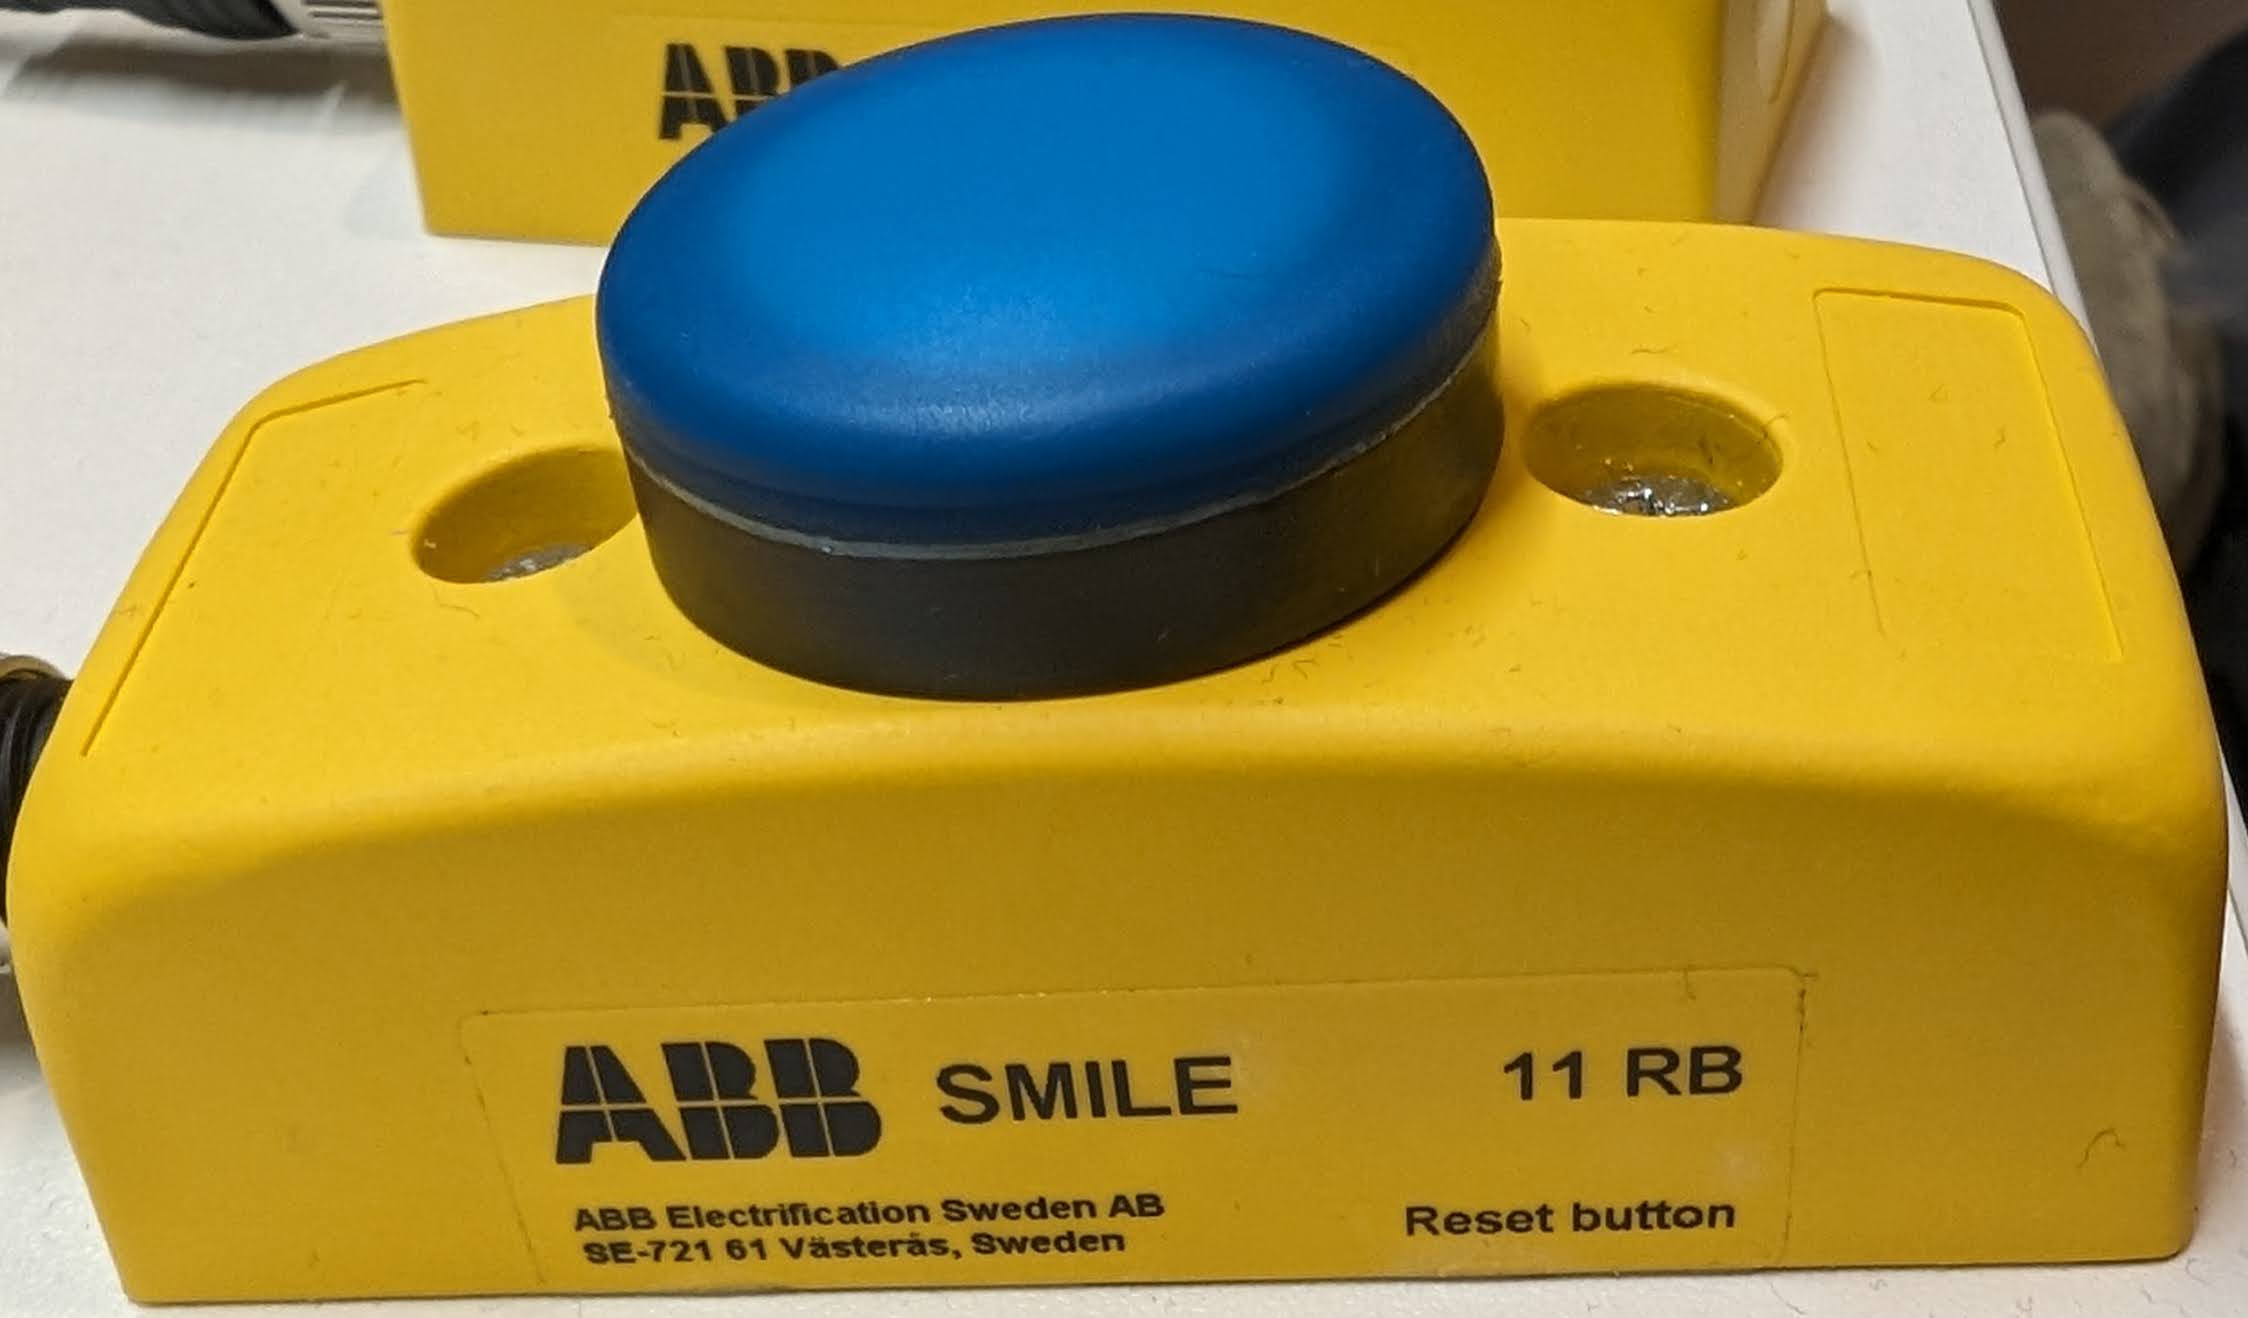
\includegraphics[width=9cm]{./lSikkerhetsPLSx01.jpg}$$
$$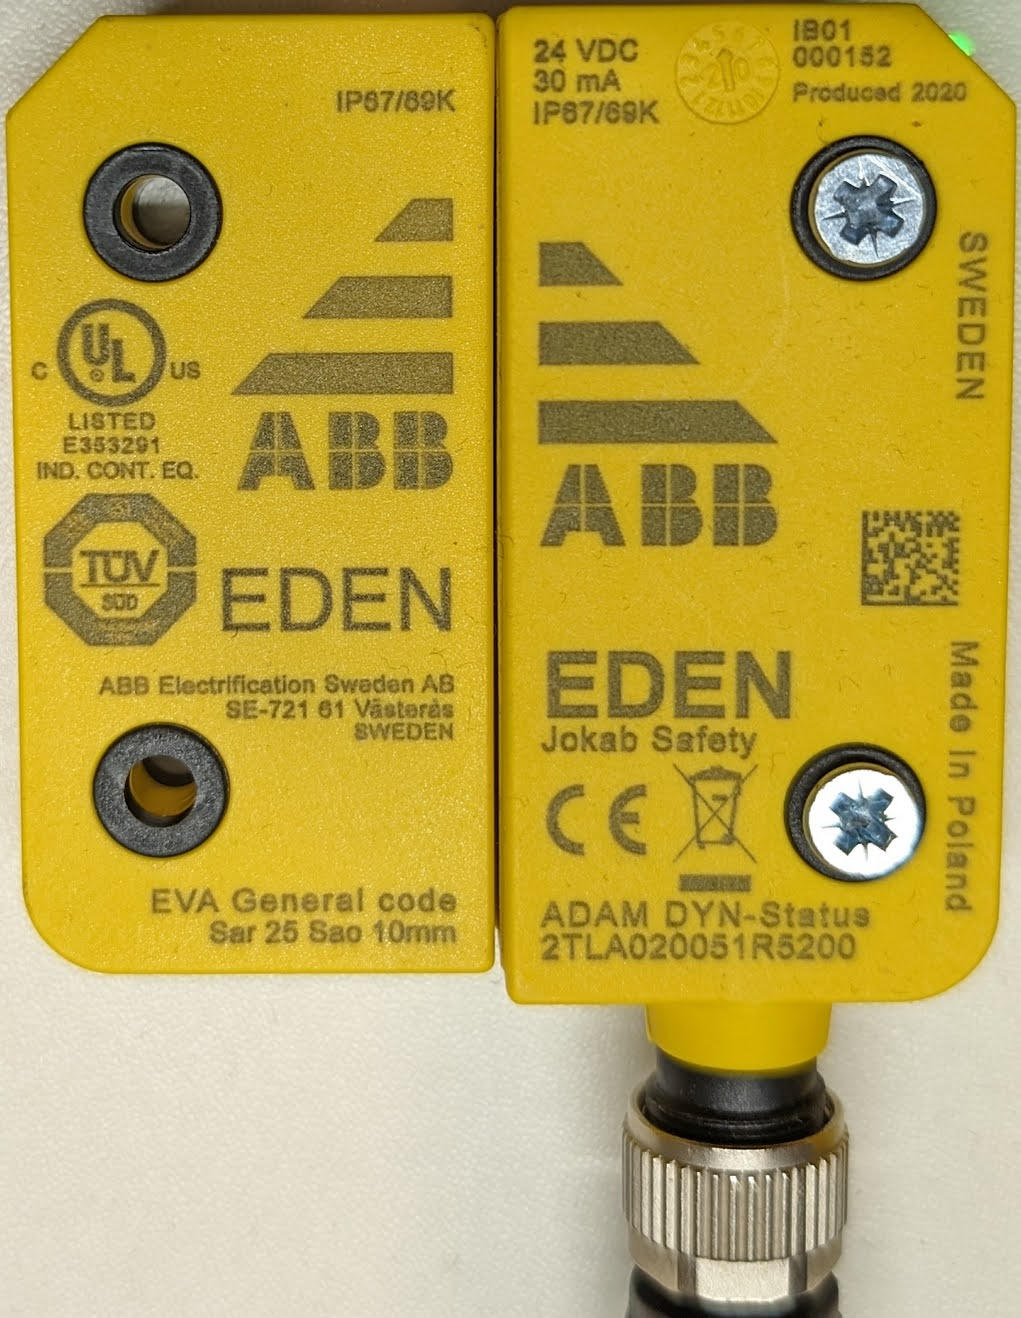
\includegraphics[width=9cm]{./lSikkerhetsPLSx02.jpg}$$
$$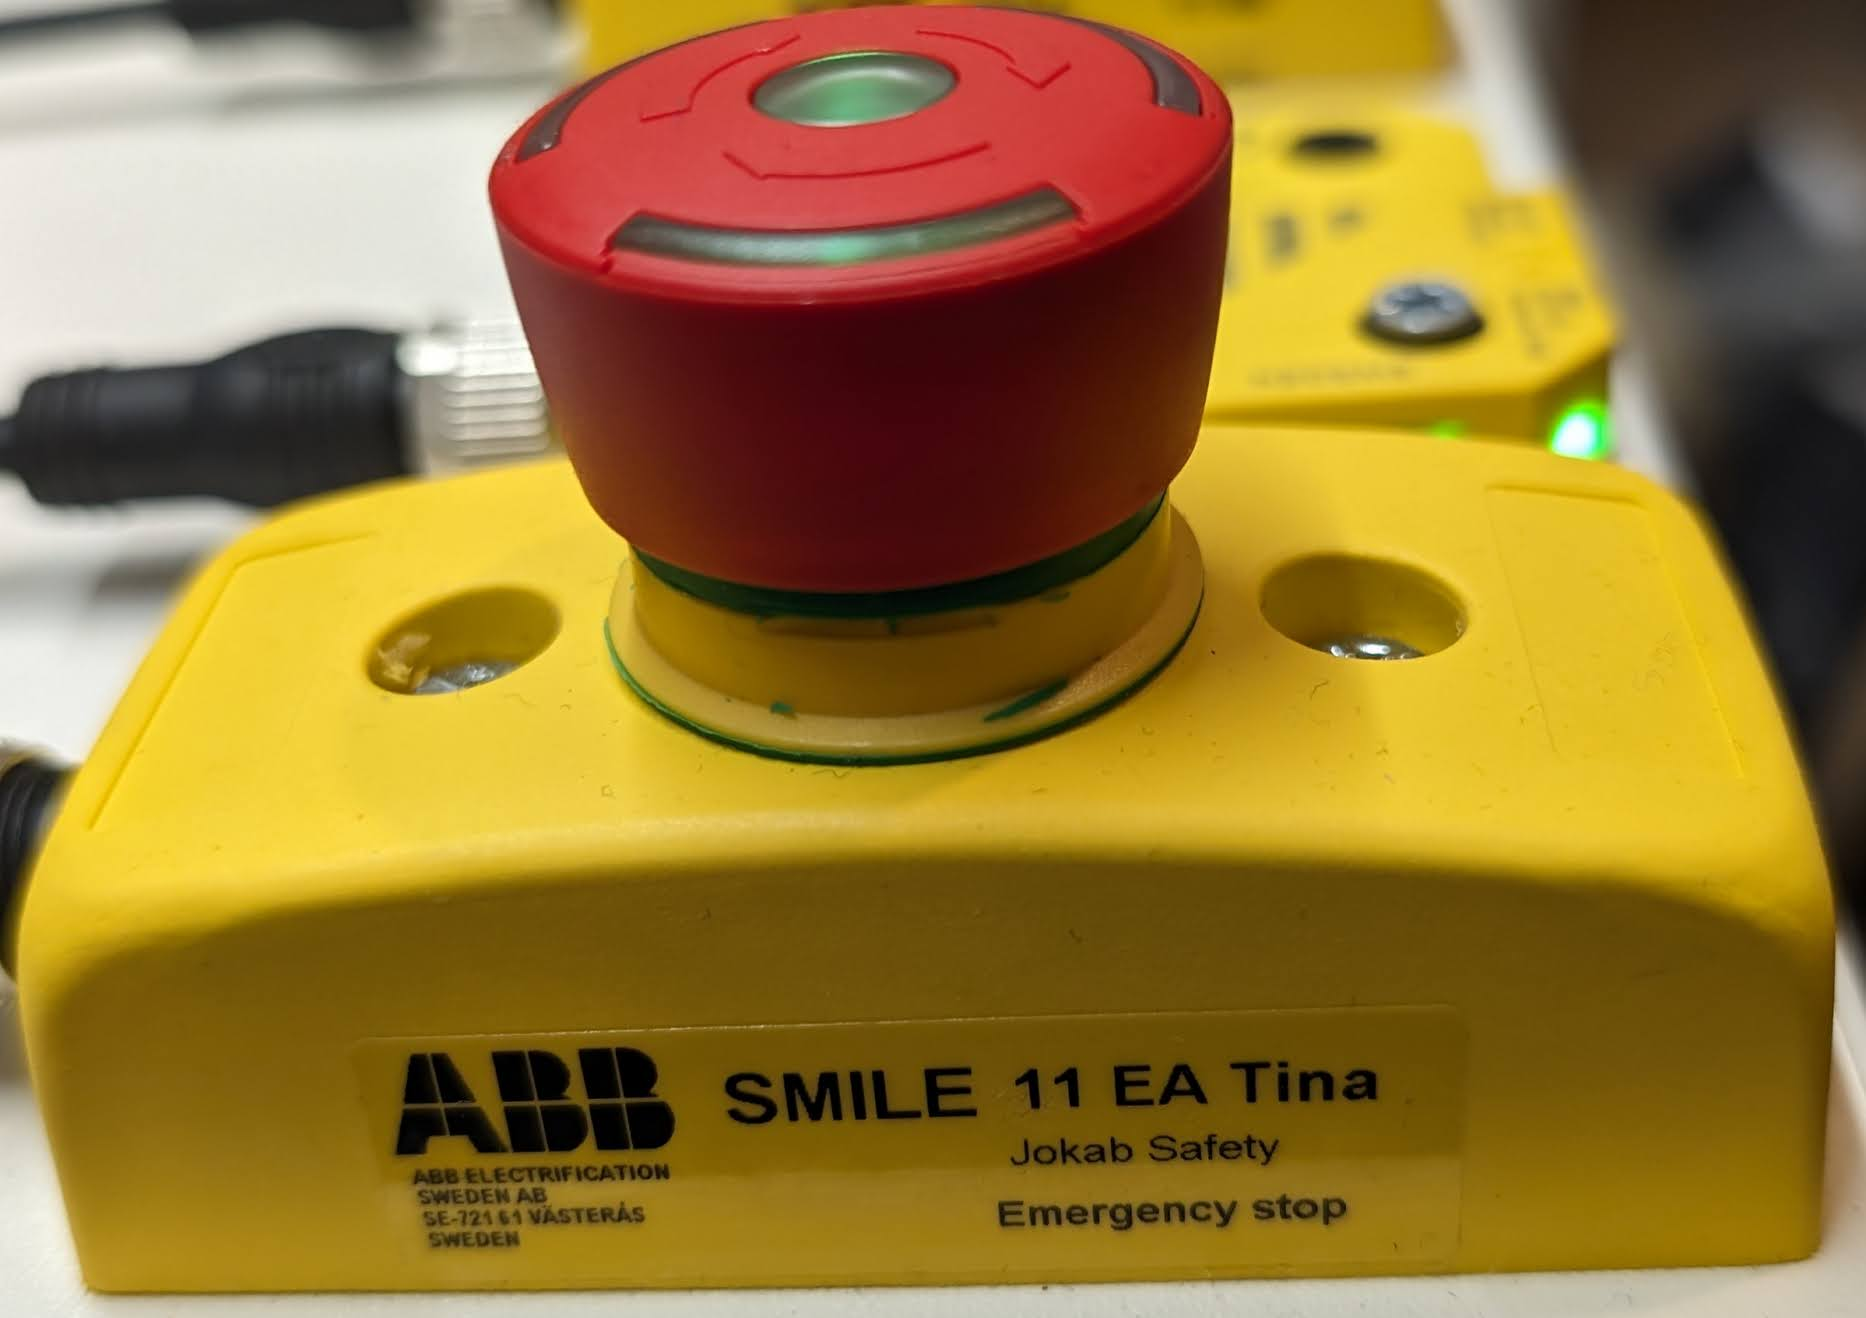
\includegraphics[width=9cm]{./lSikkerhetsPLSx03.jpg}$$
Finn manualen til disse komponentene på hjemmesiden til ABB. Lag et skjema for oppkobling til Jokab Pluto B20 v2. få læreren til å godkjenne skjema og koble opp. 
\vskip 2.5pt 

\underbar{file ./lSikkerhetsPLS.tex}
\vskip 5pt 

\end{document}

